\documentclass[12pt]{article}
\usepackage[english]{varioref}
\usepackage{setspace}
\usepackage[margin=2.54cm]{geometry}
\usepackage{pdfpages}
\usepackage[utf8]{inputenc}
\usepackage[english]{babel}
\usepackage{graphicx,subcaption}
\usepackage{graphics}
\usepackage{lscape}
\usepackage{pdflscape}
\usepackage{float}
\usepackage{textcomp}
\usepackage{amsmath}
\usepackage{hyperref}
\usepackage{fancyvrb}
\usepackage{parskip}
\usepackage{changepage}
\usepackage{enumitem}
\usepackage{tcolorbox}
\usepackage[all]{hypcap}
\usepackage{xcolor}
\usepackage{listings}
\definecolor{green}{HTML}{228B22}
\definecolor{orange}{HTML}{FFC107}
\usepackage{color}
\definecolor{dkgreen}{rgb}{0,0.6,0}
\definecolor{gray}{rgb}{0.5,0.5,0.5}
\definecolor{mauve}{rgb}{0.58,0,0.82}
\lstset{escapeinside={<@}{@>}}

\hypersetup{
    colorlinks,
    citecolor=black,
    filecolor=black,
    linkcolor=black,
    urlcolor=black
}


\lstset{frame=tb,
    language=java,
    aboveskip=3mm,
    belowskip=3mm,
    showstringspaces=false,
    columns=flexible,
    basicstyle={\small\ttfamily},
    numbers=none,
    numberstyle=\tiny\color{gray},
    keywordstyle=\color{blue},
    commentstyle=\color{dkgreen},
    stringstyle=\color{mauve},
    breaklines=true,
    breakatwhitespace=true, tabsize=3
}
\title{
	\begin{center}
	\vspace{3cm}
	\includegraphics[width=11cm, height=3cm]{Images/Logo-nou-eps.jpg}
	\end{center}
	\begin{center}
	\line(1,0){340}
	\end{center}		
	DISTRIBUTED COMPUTING\\
	\vspace{2mm}
	\Large Recent advances and new challenges \\
	\line(1,0){340}
	\vspace{2.5cm}
	}

\author{Marc Cervera Rosell - 47980320C \vspace{1cm}}


\date{Academic course 2022 - 2023\vspace{0.5cm} \\Bachelor's degree in computer engineering}
\onehalfspacing

\begin{document}
	\begin{titlepage}
		\maketitle
		\thispagestyle{empty}
	\end{titlepage}
	\cleardoublepage
	\newpage

\tableofcontents
\listoffigures
\thispagestyle{empty}

\newpage
\section*{Introduction}
\addcontentsline{toc}{section}{Introduction}
The main aim of this report is going to be to discover RabbitMQ software.\\
As everybody knows, there're three main essential attributes when designing and developing software that helps companies to offer trustworthy digital services and products. These three main attributes are: scalability, resiliency and interoperability.\\
In the actual market, there is a big amount of technologies that achieve that target. Among these technologies, we can find RabbitMQ.\\
RabbitMQ is an open-source message broker, sometimes called message-oreinted middleware.\\
This software implements the "Advanced message queuing protocol". The RabbitMQ server is programmed in Erlang and uses the "Open telecom platform" framework to build his distributed execution and error commutation capacities.\\
RabbitMQ is a cross-platform software and the source code is released under the Mozilla public license.\\
In a simplified way, RabbitMQ defines queues that will store the messages sent by producers until the consumer apps get the message and process it.\\
So, It can be said that RabbitMQ, in his broker role, has the work of routing to the correct consumer the messages that the producer sends.
To download and starting to use the software, just enter in the \href{https://www.rabbitmq.com}{\underline{RabbitMQ}} webpage.
\pagenumbering{arabic}

\section*{Architecture}
\addcontentsline{toc}{section}{Architecture}
Originally, RabbitMQ implemented the "Advanced message queuing protocol" (AMQP) but has been extended with a plug-in architecture to support "Streaming text oriented messaging protocol" (STOMP), "MQ telemetry transport" (MQTT), "HTTP and WebSockets" and "RabbitMQ streams".\\
HTTP is not really a messaging protocol but RabbitMQ can transmit messages over HTTP in three ways. The first one is the web STOMP plugin that supports STOMP messaging to the browser using WebSockets. The second one, is the web MQTT plugin that supports MQTT messaging to the browser using WebSockets. The tird, and the final, way is the management plugin that supports a simple HTTP API to send and receive messages. This is primarily intended for diagnostic purposes but can be used for low volume messaging without reliable delivery.
\newpage
\subsection*{AMQP}
\addcontentsline{toc}{subsection}{AMQP}
As AMQP is the "core" protocol supported by the broker, this section will be the most extensive.\\
RabbitMQ, originally only supported AMQP 0-9-1. All of the variants are fairly similar to each other, with later versions tidying up the unclear or unhelpful parts of earlier versions.\\
AMQP 0-9-1 is a binary protocol, and defines quite strong messaging semantics. For client it's a reasonably easy protocol to implement, and as such there are a large number of client libraries available for many different programming languages and environments.\\
AMQP is an advanced queue messaging protocol that stands out for his fidelity. There're commercial and open-source servers and interoperable clients for many programming languages, which facilitates  their use. It's used by big corporations that process millions of messages.\\
The deffinition of AMQP can be simplified in three words: "message-oriented middleware". Behind this simple definition there're a lot of features available. Before AMQP there were some message-oriented middlewares such, for example, JMS, but AMQP has become the standard protocol to keep when a queue-based solution is chosen.\\
AMQP is pretty simple to understand, there're client applications called producers that create messages and deliver it to an AMQP server, also called, broker. Inside the broker the messages are routed and filtered until arrive to queues where another applications called consumers are connected and get the messages to be processed.

\begin{figure}[H]
    \centering
    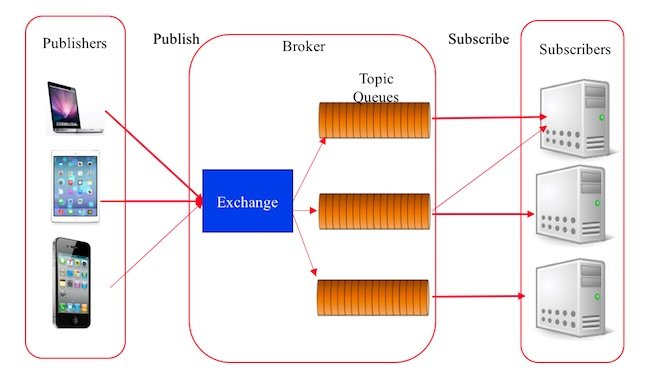
\includegraphics[scale = 0.7]{Images/AMQP-architecture-34.png}
    \caption{AMQP architecture work}
    \label{fig:AMQP_architecture}
\end{figure}

Once seen this, it's time to deep inside the broker, where the magic of AMQP is done.\\
The broker has three different parts. The exchange, the queues and the bindings.

\subsubsection*{Exchange}
\addcontentsline{toc}{subsubsection}{Exchange}
This component is in charge of receiving the messages that have been sent to the broker by a producer and is the responsible of place them in the proper queue according to a routing key. This means that the producer does not send the messages directly to the queue, but send it to an exchange with a routing key.\\
In this way, if a producer wants to send a message to various queues, does not have to send It to each one of them, but the exchange is responsible for distributing this message to each one of the queues. There're three types of exchange: direct, topic and fanout.\\

\begin{itemize}
    \item \textit{Direct exchange}: Takes the routing key that comes inside the message and sends it to the queue that's associated with this exchange and with this routing key.\\
    Example:\\
    \begin{figure}[H]
        \centering
        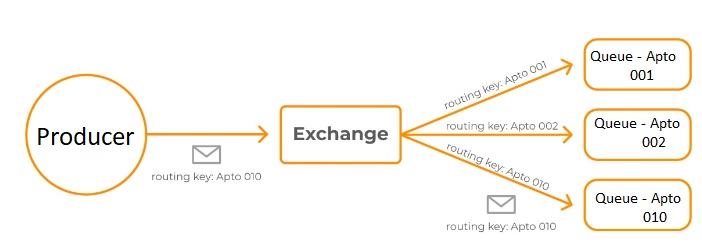
\includegraphics[scale = 0.7]{Images/direct_exchange.jpg}
        \caption{Message sending to a direct exchange}
        \label{fig:direct_exchange}
    \end{figure}
    Let's imagine the situation in what a postman has to deliver the mail to the concierge of a building and this has to put all the letters in the correspondence mailboxes. The process would be: The mail is delivered to the concierge (direct exchange)(the postman acts as the producer) and the concierge looks for the destination apartment and once the destination is found, the concierge puts the mail in the corresponding mailboxes.
    \item \textit{Topic exchange}: Carries the message to the queues that complain with a pattern in the routing key. For example, if we've the queue "Q1" associated with the exchange "EXCH1" with the routing key "gunLicense.exam.theoretical" and the queue "Q2" associated with the same exchange with the routing key "gunLicense.exam.practical", a message that's sent to the exchange "EXCH1" with the routing key "gunLicense.exam.*" will be sent to both queues.\\
    Example:\\
    \begin{figure}[H]
        \centering
        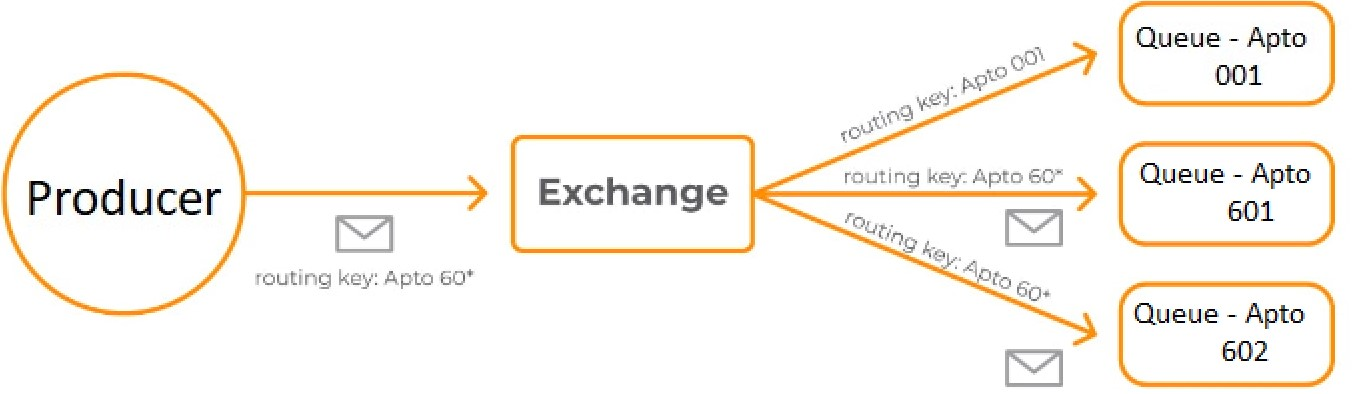
\includegraphics[scale = 0.4]{Images/topic_exchange.jpg}
        \caption{Message sending to a topic exchange}
        \label{fig:topic_exchange}
    \end{figure}
    In this case, the situation is going to change kind of. Now, the situation is: The postman will deliver to the concierge two letters (both letters are equal) that go, only, to the neighbours of the last floor (let's imagine that in the last floor are the flats 601 and 602). Hence, the postman (producer in this situation) delivers the letters to the concierge and this puts the letters inside the mailboxes, only checking (in this example) the two first numbers 6 and 0 because the digits that identify the last floor are the two first ones.
    \item \textit{Fanout exchange}: Sends the message to all the queues associated with the exchange, regardless of routing key.
    \begin{figure}[H]
        \centering
        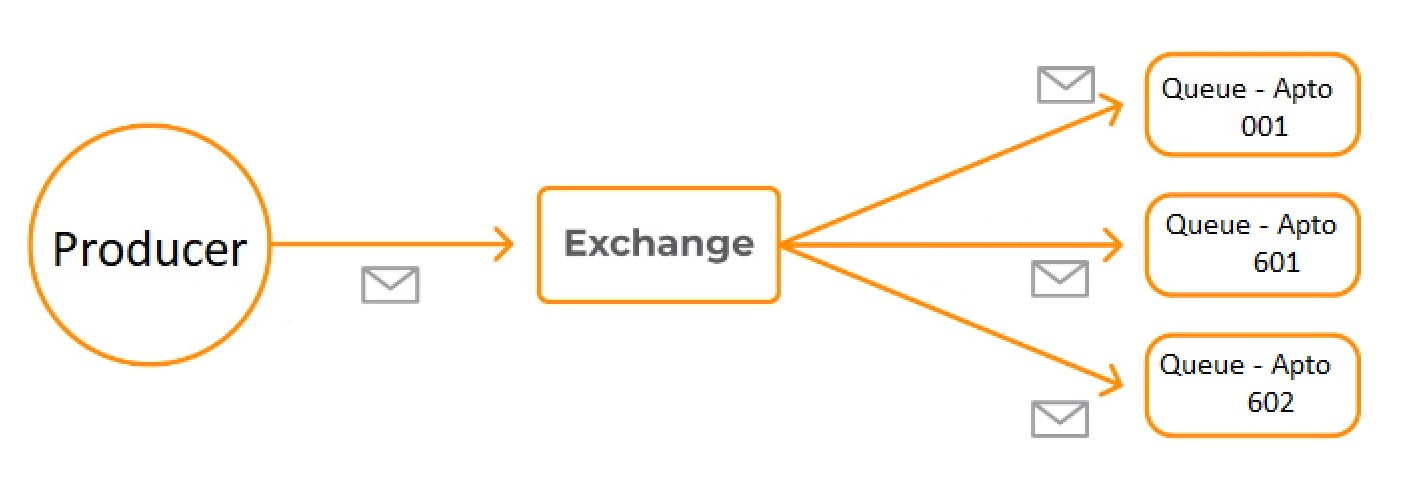
\includegraphics[scale = 0.4]{Images/fanout_exchange.jpg}
        \caption{Message sending to a topic exchange}
        \label{fig:fanout_exchange}
    \end{figure}
    \newpage
    In this final situation, the concierge will receive a letter for the entire neighbourhood. Thus, the concierge will not check neither the floor nor the flat. Instead, will put a copy of the letter in each neighbour's mailbox.
\end{itemize}

\subsubsection*{Routing key}
\addcontentsline{toc}{subsubsection}{Routing key}
Is the identifier that uses the exchange to know the route of a message. At the same time is the identifier that uses a queue to know with which exchange has to associate.

\subsubsection*{Queue}
\addcontentsline{toc}{subsubsection}{Queue}
A queue is a data structure that imitates real queues as the ones we can see in the mailbox or at the neighbourhood supermarket.
A message queue is an asynchronous communication way that's used on microservices architectures. The messages are stored in the queue until are received and deleted being every message processed only once.\\
Hence, the queue is the component that stores messages from the exchange and sends them to the consumers that are listening for these messages.

\subsubsection*{Binding}
\addcontentsline{toc}{subsubsection}{Binding}
A binding is a relationship between an exchange and a queue. This can be simply read as: the queue is interested in messages from this exchange.\\
Bindings can take an extra routing key parameter.\\
This is how a binding with a key could be created\\
\begin{lstlisting}
    channel.queue_bind(exchange = excahnge_name,
                        queue = queue_name,
                        routing_key = 'black')
\end{lstlisting}
The above code, is using the \textit{Pika} Python client.\\
The meaning of a binding key depends on the exchange type. The \textit{fanout} exchanges, just ignore this value.

\subsubsection*{Virtual host}
\addcontentsline{toc}{subsubsection}{Virtual host}
RabbitMQ is multy-tenant system: connections, exchanges, queues, bindings and some other things belong to virtual hosts. If the user is familiar with virtual hosts in Apache, the idea is similar. However, there's an important difference: in Apache, virtual hosts are defined in the configuration file; that's no the case of RabbitMQ; virtual hosts are created and deleted using \textit{rebbitmqctl} or HTTP API instead.\\
A virtual host, provides logical grouping and separation resources. Separation of physical resources is not a goal of virtual hosts and should be considered an implementation detail.\\
For example, resource permissions in RabbitMQ are scoped per virtual host. A user does not have global permissions, only permissions in one or more virtual hosts. User tags can be considered global permissions but they are an exception to the rule.\\
Therefore when talking about user permissions it's very important to clarify what virtual host(s) they apply to.\\
A virtual host has a name. When an AMQP 0-9-1 client connects to RabbitMQ, it specifies a virtual host name to connect to. If the username is not granted permissions, the connection is refused.

\paragraph*{Creating and deleting virtual hosts\\}
\textit{Using CLI tools:\\}
\begin{lstlisting}
    rabbitmqctl add_vhost qua1
\end{lstlisting}

\begin{lstlisting}
    rabbitmqctl delete_vhost qua1
\end{lstlisting}

\textit{Using HTML API\\}
\begin{lstlisting}
    curl -u username:pa$sw0rD -X PUT http://rabbitmq.local:15672/api/vhosts/vh1
\end{lstlisting}

\begin{lstlisting}
    curl -u username:pa$sw0rD -X DELETE http://rabbitmq.local:15672/api/vhosts/vh1
\end{lstlisting}

\section*{Applications}
\addcontentsline{toc}{section}{Applications}
In this section of the report, some messaging protocols will be seen, but they have been placed here because, in the RabbitMQ context, all of them are plugins. This means that, RabbitMQ can work properly without this set of protocols and if It can work means that these protocols are not mandatory, nevertheless, AMQP is completely mandatory for RabbitMQ.
If we have to distinguish, easily, between architecture and applications, we could say that architecture are those protocols that are completely necessary for running the software and applications are other things that the software can run properly without. This is the reason because in this section protocols like MQTT and STOMP will be seen.
\subsection*{MQTT}
\addcontentsline{toc}{subsection}{MQTT}
MQTT is M2M communication protocol of type message queue.\\
It's based on the TCP stack as the communication base. In the MQTT case, every connection keeps opened and is “reused” in every communication. It's a difference, for example, with an HTTP 1.0 petition where every transmission is reused through the connection.\\
MQTT was created by Dr. Andy Stanford-Clark of IBM and Arlen Nipper de Arcom in 1999 as a mechanism to connect devices used in the petrol industry.\\
Though initially was a proprietary format, in 2010 was released and in 2014, became a standard according to OASIS (Organization for the Advancement of Structured Information Standards).\\
The MQTT work is a push messaging service with the pub-sub pattern. In this type of infrastructures, the clients they connect with a central server named broker.\\
To filter the messages that are sent to each client, the messages are arranged in topics hierarchically organized. A client can publish a message in a specific topic. Other clients can subscribe to this topic and the broker will send the subscribed messages.

\begin{figure}[H]
    \centering
    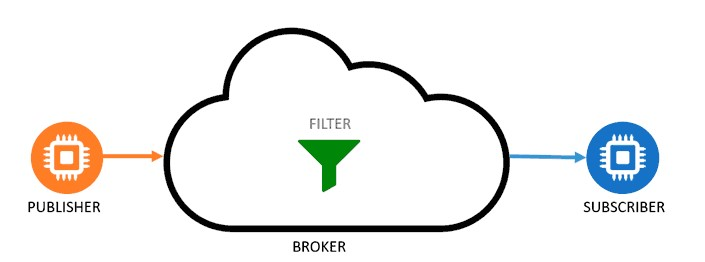
\includegraphics[scale = 0.7]{Images/mqtt.jpg}
    \caption{MQTT}
    \label{fig:mqtt}
\end{figure}

The clients start a TCP/IP connection with the broker, which maintain a registration of the connected clients. This connection keeps opened until the client ends it. By default, MQTT uses the ports 1883 and 8883 when works on TLS.\\
To do that, the client sends a CONNECT message that contains the necessary information. The broker answers with a CONNACK message, that contains the result of the connection.\\
To send the messages, the client uses PUBLISH messages, that contain the topic and the payload.\\
To subscribe and unsubscribe, the SUBSCRIBE and UNSUBSCRIBE messages are used. The server responds with a SUBACK or with a UNSUBACK.\\
To make sure that the connection is active, the clients send periodically a PINGREQ message which is answered, by the server, with a PINGRESP, Finally, the client disconnects sending a DISCONNECT message.\\
\begin{figure}[H]
    \centering
    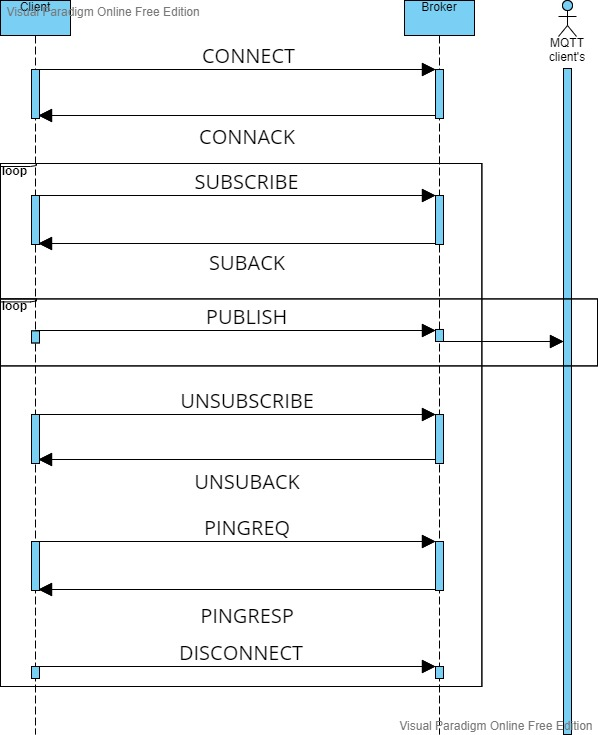
\includegraphics[scale = 0.6]{Images/DSS RabbitMQ.jpg}
    \caption{Working example of MQTT}
    \label{fig:mqtt_example}
\end{figure}
To anable the MQTT plugin:
\begin{lstlisting}
    rabbitmq-plugins enable rabbitmq_mqtt
\end{lstlisting}

\subsection*{STOMP}
\addcontentsline{toc}{subsection}{STOMP}
STOMP is the Simple Text Oriented Messaging Protocol.\\
STOMP provides an interoperable wire format so that STOMP clients can communicate with any STOMP message broker to provide easy and widespread messaging interoperability among many languages, platforms and brokers\\
STOMP is a very simple and easy to implement protocol, coming from the HTTP school of design; the server side may be hard to implement well, but it is very easy to write a client to get yourself connected.\\
Many developers have told that they have managed to write a STOMP client in a couple of hours to in their particular language, runtime or platform into the STOMP network.\\
To anable the STOMP plugin:
\begin{lstlisting}
    rabbitmq-plugins enable rabbitmq_stomp
\end{lstlisting}

\subsection*{WebSockets}
\addcontentsline{toc}{subsection}{WebSockets}
As it has been said before, RabbitMQ can transmit messages over HTTP in three ways, and tow of these are using WebSockets. These two ways are plugins; the first one supports STOMP messaging and the second supports MQTT.\\
To enable the STOMP WebSocket plugin:
\begin{lstlisting}
    rabbitmq-plugins enable rabbitmq_web_stomp
\end{lstlisting}
To enable the MQTT WebSocket plugin:
\begin{lstlisting}
    rabbitmq-plugins enable rabbitmq_web_mqtt
\end{lstlisting}

\subsection*{RabbitMQ streams}
\addcontentsline{toc}{subsection}{RabbitMQ streams}
The RabbitMQ streams protocol allows communicating with streams.\\
The RabbitMQ stream is a Java library to communicate with the RabbitMQ Stream plugin. It allows creating and delete streams, as well as to publish to and consume from these streams. The protocol is still under development and is subject to change.\\
To enable the RabbitMQ streams plugin:
\begin{lstlisting}
    rabbitmq-plugins enable rabbitmq_stream
\end{lstlisting}

\subsubsection*{Streams}
\addcontentsline{toc}{subsubsection}{Streams}
A stream is a sequence of elements from a source that supports data processing operations.\\
Sequence of elements: while collections are about data, streams are about computations.\\
Source: Streams consume data from a providing source.\\
Data processing operations:

\begin{itemize}
    \item Database-like and functional programming.
    \item Pipelining and internal iteration
\end{itemize}

\section*{RabbitMQ in the  market}
\addcontentsline{toc}{section}{RabbitMQ in the market}
This report's section is going to contain three parts. In the first one, will be shown the advantages of using RabbitMQ. In the second one, on the contrary, will be shown the disadvantages of this technology and in the final section is going to be mentioned the most important competition in the market.

\subsection*{Advantages}
\addcontentsline{toc}{subsection}{Advantages}
\begin{enumerate}
    \item Allows the integration of different applications through messages in an asynchronous way (decoupling in time) and from various locations (decoupling in space).
    \item Reliability: RabbitMQ incorporates several characteristics that allow it to guarantee the delivery of the messages. Among them, provides storing when there's no available consumers to receive the message, offers the possibility that the consumer accepts the delivery of the message to make sure that it has been processed successful and, in case the prosecution has failed, allows the message can be re-queued for being consumed by a different instance of the consumer or be processed again by the same consumer (the one that initially failed), when this recovers.\\
    RabbitMQ, guarantees the order of delivery, it's to say, the messages are consumed in the same order in which they have arrived at the queues.
    \item Cluster creation: while RabbitMQ provides high-performance processing thousands of messages per second, sometimes has to be able to process more messages without impacting on the application's performance. For this, RabbitMQ allows the creation of clusters to scale horizontally the solution. This is transparent for the producers and for the consumers.
     \item Available: In RabbitMQ, the queues can be replicated in several nodes of the cluster, providing the security that in case of failure of a node the broker can keep receiving messages of the producers and keep delivering them to the proper consumers.
    \item Security: RabbitMQ has inbuilt to support the Transport Layer Security (TLS) protocol. TLS is a cryptographic protocol that provides secure connections through a network, commonly the Internet. TLS uses X.509 certificates and therefore asymmetric cryptography to authenticate the counterpart who are they communicating and to exchange a symmetric key. Hence, it can be said that RabbitMQ has a good security level.
    \item Affordability: As RabbitMQ is an open-source software, the affordability is complete. In other words, RabbitMQ is totally free, therefore is completely affordable for those persons that have enough resources to buy a computer and contract an internet plan.
    \item Failure tolerance: As it can be seen in the following image, RabbitMQ has a simple but fruitful failure handler system:
    \begin{figure}[H]
        \centering
        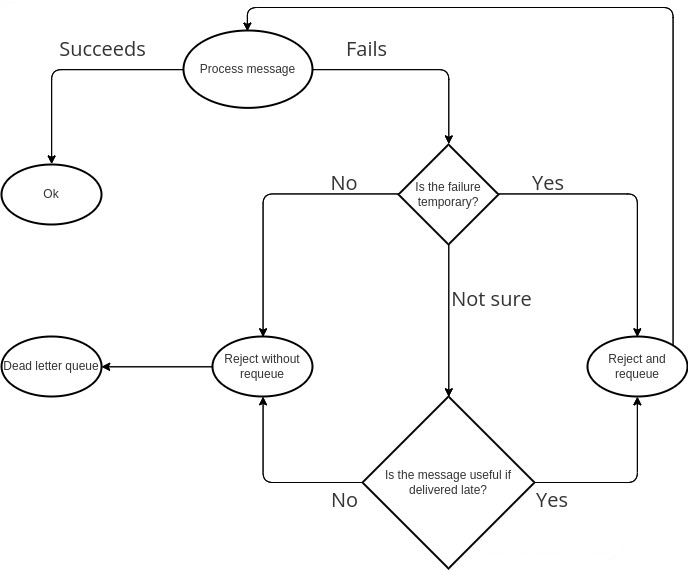
\includegraphics[scale = 2]{Images/fault handling process.jpg}
        \caption{RabbitMQ's failure handler system}
        \label{fig:failure}
    \end{figure}
    \item Complexity: RabbitMQ is user-friendly and it's easy to modify the configurations to suit the expected porpouse. RabbitMQ is written in Erlang and it's the world's most deployed open-source message broker, meaning that it's a well-tested and robust message broker.
    \item Latency: Has the lowest latency of the market.
    \item Performance: Has one of the best yields of the market.
\end{enumerate}

\subsection*{Disadvantages}
\addcontentsline{toc}{subsection}{Disadvantages}
\begin{enumerate}
    \item Latency: The consumers will balloon in memory as they buffer all the messages in their own RAM. A big buffer, results in a lot of extra latency if the network performs normally, and huge amounts of extra latency if the client suddenly starts taking longer to process each message than normal.
    \item Resource sharing: Firstly, It has to be said that for allowing resource sharing in RabbitMQ, the management plugin has to be enabled. Secondly, if the plugin is enabled, by default the management UI application will refuse to access to websites hosted on origins different from its own using the CORS mechanism. It is possible to allow any origin to use the API using a wildcard. This is highly discouraged for deployments where the UI application may be exposed to the public.\\
    The wildcard is:\\
    \begin{lstlisting}
        management.cors.allow_origins.1 = *
    \end{lstlisting}
    The counsel is to allow the origins different by its own one by one, as it can be seen in the bottom code fragment:
    \begin{lstlisting}
        management.cors.allow_origins.1 = https://www.origin1.org
        management.cors.allow_origins.2 = https://www.origin2.org
    \end{lstlisting}
    \item High resource usage: As it has been seen, AMQP is RabbitMQ's core protocol and AMQP has a big disadvantage: the resource consumption. The AMQP clients need a certain processing capacity. It's not intended for its implementation in devices with few computational resources. Furthermore, because of the big quantity of control traffic that is introduced to offer reliability, it's not meant for its implementation in networks with low bandwidth.
    \item RabbitMQ is developed in Erlang, which makes difficult to understand.
\end{enumerate}

\subsection*{Competition on the market}
\addcontentsline{toc}{subsection}{Competition on the market}
This section will contain a few examples of RabbitMQ's market competition.
\begin{itemize}
    \item Memphis
    \begin{figure}[H]
        \centering
        
\includegraphics[scale = 0.5]{Images/memphis.jpeg}
        \caption{Memphis' logo}
        \label{fig:memphis}
    \end{figure}
    \newpage
    \item Apache Kafka
    \begin{figure}[H]
        \centering
        
\includegraphics[scale = 0.4]{Images/kafka.jpg}
        \caption{Apache kafka's logo}
        \label{fig:kafka}
    \end{figure}
    \item Apache ActiveMQ
    \begin{figure}[H]
        \centering
        
\includegraphics{Images/active.jpg}
        \caption{Apache ActiveMQ's logo}
        \label{fig:activemq}
    \end{figure}
    \item WSO2
    \begin{figure}[H]
        \centering
        
\includegraphics[scale = 0.7]{Images/WSO2.png}
        \caption{WSO2's logo}
        \label{fig:wso2}
    \end{figure}
    \newpage
    \item ZeroMQ
    \begin{figure}[H]
        \centering
        
\includegraphics[scale = 0.7]{Images/zeromq-logo.jpg}
        \caption{ZeroMQ's logo}
        \label{fig:zeromq}
    \end{figure}
\end{itemize}

\section*{Conclusions}
\addcontentsline{toc}{section}{Conclusions}
\begin{enumerate}
    \item RabbitMQ has a core architecture, but can support others through plugins.
    \item RabbitMQ is uncomplicated to use, reliable, scalable, available, secure, affordable, fault-tolerant, and efficient.
    \item As AMQP supports many programming languages to be implemented, there are many libraries available to implement the protocol in many ways.
    \item The exchange is a key element for the messages to arrive at the correct destination.
    \item Every message has an 'id' that makes it unique.
    \item So many similarities can be found between Apache virtual hosts' and RabbitMQ virtual hosts'.
    \item RabbitMQ is not perfect, but the advantages of using it outweighs the disadvantages.
    \item RabbitMQ has a lot of market competition, but is the most chosen by the companies.
\end{enumerate}

\section*{References}
\addcontentsline{toc}{section}{References}
\begin{itemize}
    \item \href{https://en.wikipedia.org/wiki/RabbitMQ}{\underline{Wikipedia's RabbitMQ article}}
    \item \href{https://www.rabbitmq.com}{\underline{RabbitMQ's webpage}}
    \item \href{https://www.sdos.es/blog/microservicios-mensajes-spring-rabbitmq}{\underline{\textit{Conectar microservicios con colas de mensajes usando Spring y RabbitMQ}'s webpage}}
    \item \href{https://www.pragma.com.co/academia/lecciones/conozcamos-sobre-rabbitmq-sus-componentes-y-beneficios}{\underline{\textit{Conozcamos sobre RabbitMQ, sus componentes y beneficios}'s webpage}}
    \item \href{https://www.researchgate.net/publication/325119432/figure/fig5/AS:626093459505153@1526283721309/AMQP-architecture-34.png}{\underline{AMQP architecture work picture}}
    \item \href{https://www.rabbitmq.com/protocols.html}{\underline{Which protocols does RabbitMQ support?}}
    \item \href{https://www.rabbitmq.com/vhosts.html}{\underline{Creating and deleting virtual hosts}}
    \item \href{https://www.luisllamas.es/que-es-mqtt-su-importancia-como-protocolo-iot/}{\underline{MQTT}}
    \item \href{https://en.wikipedia.org/wiki/WebSocket}{\underline{WebSocket wikipedia's page}}
    \item \href{http://stomp.github.io}{\underline{STOMP}}
    \item \href{https://programmerclick.com/article/80671335987/}{\underline{Advantages and disavantages of RabbitMQ}}
    \item \href{https://blog.devgenius.io/scalable-system-implementation-using-rabbitmq-java-and-mysql-2d5fe0fa182e}{\underline{RabbitMQ properties}}
    \item \href{https://blog.rabbitmq.com/posts/2012/05/some-queuing-theory-throughput-latency-and-bandwidth/}{\underline{Some queuing theory: throughput, latency and bandwidth}}
    \item \href{https://medium.com/codait/handling-failure-successfully-in-rabbitmq-22ffa982b60f}{\underline{Handling failure successfully in RabbitMQ}}
    \item \href{https://www.rabbitmq.com/management.html}{\underline{RabbitMQ's management plugin}}
    \item \href{https://geekflare.com/es/top-message-brokers/}{\underline{RabbitMQ's market competition}}
    \end{itemize}
\end{document}